% Options for packages loaded elsewhere
\PassOptionsToPackage{unicode}{hyperref}
\PassOptionsToPackage{hyphens}{url}
%
\documentclass[
  a4paper,
]{article}
\usepackage{amsmath,amssymb}
\usepackage{setspace}
\usepackage{iftex}
\ifPDFTeX
  \usepackage[T1]{fontenc}
  \usepackage[utf8]{inputenc}
  \usepackage{textcomp} % provide euro and other symbols
\else % if luatex or xetex
  \usepackage{unicode-math} % this also loads fontspec
  \defaultfontfeatures{Scale=MatchLowercase}
  \defaultfontfeatures[\rmfamily]{Ligatures=TeX,Scale=1}
\fi
\usepackage{lmodern}
\ifPDFTeX\else
  % xetex/luatex font selection
\fi
% Use upquote if available, for straight quotes in verbatim environments
\IfFileExists{upquote.sty}{\usepackage{upquote}}{}
\IfFileExists{microtype.sty}{% use microtype if available
  \usepackage[]{microtype}
  \UseMicrotypeSet[protrusion]{basicmath} % disable protrusion for tt fonts
}{}
\makeatletter
\@ifundefined{KOMAClassName}{% if non-KOMA class
  \IfFileExists{parskip.sty}{%
    \usepackage{parskip}
  }{% else
    \setlength{\parindent}{0pt}
    \setlength{\parskip}{6pt plus 2pt minus 1pt}}
}{% if KOMA class
  \KOMAoptions{parskip=half}}
\makeatother
\usepackage{xcolor}
\usepackage[margin=1in]{geometry}
\usepackage{color}
\usepackage{fancyvrb}
\newcommand{\VerbBar}{|}
\newcommand{\VERB}{\Verb[commandchars=\\\{\}]}
\DefineVerbatimEnvironment{Highlighting}{Verbatim}{commandchars=\\\{\}}
% Add ',fontsize=\small' for more characters per line
\usepackage{framed}
\definecolor{shadecolor}{RGB}{248,248,248}
\newenvironment{Shaded}{\begin{snugshade}}{\end{snugshade}}
\newcommand{\AlertTok}[1]{\textcolor[rgb]{0.94,0.16,0.16}{#1}}
\newcommand{\AnnotationTok}[1]{\textcolor[rgb]{0.56,0.35,0.01}{\textbf{\textit{#1}}}}
\newcommand{\AttributeTok}[1]{\textcolor[rgb]{0.13,0.29,0.53}{#1}}
\newcommand{\BaseNTok}[1]{\textcolor[rgb]{0.00,0.00,0.81}{#1}}
\newcommand{\BuiltInTok}[1]{#1}
\newcommand{\CharTok}[1]{\textcolor[rgb]{0.31,0.60,0.02}{#1}}
\newcommand{\CommentTok}[1]{\textcolor[rgb]{0.56,0.35,0.01}{\textit{#1}}}
\newcommand{\CommentVarTok}[1]{\textcolor[rgb]{0.56,0.35,0.01}{\textbf{\textit{#1}}}}
\newcommand{\ConstantTok}[1]{\textcolor[rgb]{0.56,0.35,0.01}{#1}}
\newcommand{\ControlFlowTok}[1]{\textcolor[rgb]{0.13,0.29,0.53}{\textbf{#1}}}
\newcommand{\DataTypeTok}[1]{\textcolor[rgb]{0.13,0.29,0.53}{#1}}
\newcommand{\DecValTok}[1]{\textcolor[rgb]{0.00,0.00,0.81}{#1}}
\newcommand{\DocumentationTok}[1]{\textcolor[rgb]{0.56,0.35,0.01}{\textbf{\textit{#1}}}}
\newcommand{\ErrorTok}[1]{\textcolor[rgb]{0.64,0.00,0.00}{\textbf{#1}}}
\newcommand{\ExtensionTok}[1]{#1}
\newcommand{\FloatTok}[1]{\textcolor[rgb]{0.00,0.00,0.81}{#1}}
\newcommand{\FunctionTok}[1]{\textcolor[rgb]{0.13,0.29,0.53}{\textbf{#1}}}
\newcommand{\ImportTok}[1]{#1}
\newcommand{\InformationTok}[1]{\textcolor[rgb]{0.56,0.35,0.01}{\textbf{\textit{#1}}}}
\newcommand{\KeywordTok}[1]{\textcolor[rgb]{0.13,0.29,0.53}{\textbf{#1}}}
\newcommand{\NormalTok}[1]{#1}
\newcommand{\OperatorTok}[1]{\textcolor[rgb]{0.81,0.36,0.00}{\textbf{#1}}}
\newcommand{\OtherTok}[1]{\textcolor[rgb]{0.56,0.35,0.01}{#1}}
\newcommand{\PreprocessorTok}[1]{\textcolor[rgb]{0.56,0.35,0.01}{\textit{#1}}}
\newcommand{\RegionMarkerTok}[1]{#1}
\newcommand{\SpecialCharTok}[1]{\textcolor[rgb]{0.81,0.36,0.00}{\textbf{#1}}}
\newcommand{\SpecialStringTok}[1]{\textcolor[rgb]{0.31,0.60,0.02}{#1}}
\newcommand{\StringTok}[1]{\textcolor[rgb]{0.31,0.60,0.02}{#1}}
\newcommand{\VariableTok}[1]{\textcolor[rgb]{0.00,0.00,0.00}{#1}}
\newcommand{\VerbatimStringTok}[1]{\textcolor[rgb]{0.31,0.60,0.02}{#1}}
\newcommand{\WarningTok}[1]{\textcolor[rgb]{0.56,0.35,0.01}{\textbf{\textit{#1}}}}
\usepackage{longtable,booktabs,array}
\usepackage{calc} % for calculating minipage widths
% Correct order of tables after \paragraph or \subparagraph
\usepackage{etoolbox}
\makeatletter
\patchcmd\longtable{\par}{\if@noskipsec\mbox{}\fi\par}{}{}
\makeatother
% Allow footnotes in longtable head/foot
\IfFileExists{footnotehyper.sty}{\usepackage{footnotehyper}}{\usepackage{footnote}}
\makesavenoteenv{longtable}
\usepackage{graphicx}
\makeatletter
\def\maxwidth{\ifdim\Gin@nat@width>\linewidth\linewidth\else\Gin@nat@width\fi}
\def\maxheight{\ifdim\Gin@nat@height>\textheight\textheight\else\Gin@nat@height\fi}
\makeatother
% Scale images if necessary, so that they will not overflow the page
% margins by default, and it is still possible to overwrite the defaults
% using explicit options in \includegraphics[width, height, ...]{}
\setkeys{Gin}{width=\maxwidth,height=\maxheight,keepaspectratio}
% Set default figure placement to htbp
\makeatletter
\def\fps@figure{htbp}
\makeatother
\setlength{\emergencystretch}{3em} % prevent overfull lines
\providecommand{\tightlist}{%
  \setlength{\itemsep}{0pt}\setlength{\parskip}{0pt}}
\setcounter{secnumdepth}{-\maxdimen} % remove section numbering
\ifLuaTeX
\usepackage[bidi=basic]{babel}
\else
\usepackage[bidi=default]{babel}
\fi
\babelprovide[main,import]{catalan}
% get rid of language-specific shorthands (see #6817):
\let\LanguageShortHands\languageshorthands
\def\languageshorthands#1{}
\ifLuaTeX
  \usepackage{selnolig}  % disable illegal ligatures
\fi
\usepackage{bookmark}
\IfFileExists{xurl.sty}{\usepackage{xurl}}{} % add URL line breaks if available
\urlstyle{same}
\hypersetup{
  pdftitle={U6. GESTIÓ D'USUARIS I GRUPS},
  pdfauthor={@tofermos 2024},
  pdflang={ca-ES},
  hidelinks,
  pdfcreator={LaTeX via pandoc}}

\title{U6. GESTIÓ D'USUARIS I GRUPS}
\author{@tofermos 2024}
\date{}

\begin{document}
\maketitle

{
\setcounter{tocdepth}{2}
\tableofcontents
}
\setstretch{1.5}
\newpage
\renewcommand\tablename{Tabla}

\section{1 Resum}\label{resum}

En esta unitat aprendrem com crear, modificar i eliminar comptes locals
(usuaris i grups) de Linux des de l'entorn gràfic i des de terminal.
Haurem de ser capaços de dominar:

\begin{itemize}
\tightlist
\item
  La gestió des de l'entorn GUI
\item
  La gestió amb ordres Linux
\item
  Conéixer alguns fitxers de configuració
\item
  Conéixer el perfil dels usuaris
\end{itemize}

\section{2 Consideracions prèvies}\label{consideracions-pruxe8vies}

\begin{itemize}
\tightlist
\item
  Comptes = usuaris + grups.
\item
  El permís es dona a comptes sobre carpetes o fitxers.
\item
  Un usuari pot pertanyer a més d'un grup.
\item
  Si un usuari pertany a més d'un grup té els permisos i drets que tenen
  tots els grups.
\item
  Un usuari pot fer canvis sobre la seua configuració, però no pot
  canviar-se de grup si no es administrador (sudoer)
\end{itemize}

\begin{longtable}[]{@{}lllll@{}}
\toprule\noalign{}
PC & Grup & Usuari & Permisos & Carpeta \\
\midrule\noalign{}
\endhead
\bottomrule\noalign{}
\endlastfoot
PC\_Mostrador & tornDia & Pere, Joana & /home/DirectoriAlbarans2024 &
lectura \\
& tornVesprada & Aitana, Vicent, Joana & & lectura i escriure \\
\end{longtable}

Sobre la carpeta \emph{/home/DirectoriAlbarans2024} els usuaris
podran\ldots{} Pere i Joana podran llegir el contigut de la carpeta (ls
.) i el contingut del fitxers que hi haja (cat, tail\ldots). Els usuaris
Aitana, Vicent i (també) Joana podran, llegir, crear i eliminar (touch,
cp, rm\ldots) fitxers a la carpeta i també modificar el contingut dels
fitxers.

(Assumim que els permisos dels fitxers son els mateixos que els de la
carpeta i que podem navegar (permís d'execució) per ella)

\section{3 Gestió des del GUI}\label{gestiuxf3-des-del-gui}

Observem que els UID son els identificador únics d'usuari (com un NIA,
DNI, NUSS o adreça MAC):

\begin{itemize}
\tightlist
\item
  Els usuaris que inicien sessió (persones) comença per 1000 per
  defecte.
\item
  Els usuari que corresponen a software de sistema (servicis), tenen
  valors distints.
\item
  L'usuari vboxadd i el grup són de VirtualBox, no els trobareu en
  instal·lacions normals.
\end{itemize}

Si no indiquem grup, en crea un amb el mateix nom que l'usuari assigna
un GID (major que 1000 també).

\begin{figure}
\centering
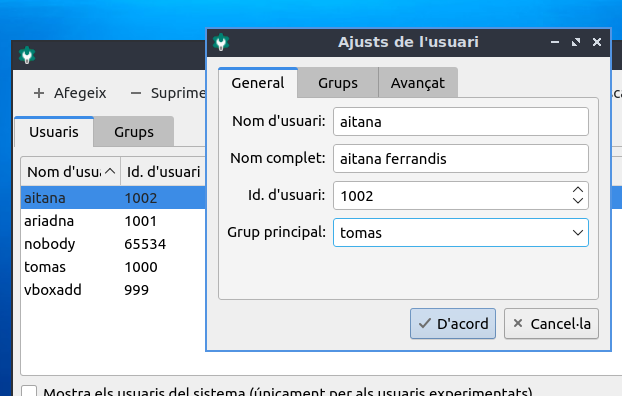
\includegraphics{png/usuarisGUI1.png}
\caption{Figura1:Usuario. Login}
\end{figure}

Podem incloure en més d'un grup.

Un grup interessant per compartir informació entre màquines (virtuals o
reals) és el \emph{sambashare}. La compartició de carpetes i fitxers
entre ordinadors (xarxa local) es veu en el mòdul de SOX. No obstant,
podrem fer alguna prova més avant.

\begin{quote}
Nota:
\end{quote}

\begin{quote}
No hem de confondre la compartició en xarxa de la compartició local en
VirtualBox
\end{quote}

En l'àmbit de màquines virtuals, tenim el \emph{vboxadd} que ens fa
falta per poder usar ``carpetes compartides'' entre la MV i el PC
amfitrió.

\begin{longtable}[]{@{}
  >{\raggedright\arraybackslash}p{(\columnwidth - 4\tabcolsep) * \real{0.2793}}
  >{\raggedright\arraybackslash}p{(\columnwidth - 4\tabcolsep) * \real{0.3604}}
  >{\raggedright\arraybackslash}p{(\columnwidth - 4\tabcolsep) * \real{0.3604}}@{}}
\toprule\noalign{}
\begin{minipage}[b]{\linewidth}\raggedright
Aspecte
\end{minipage} & \begin{minipage}[b]{\linewidth}\raggedright
Compartició general
\end{minipage} & \begin{minipage}[b]{\linewidth}\raggedright
Compartició en VirtualBox
\end{minipage} \\
\midrule\noalign{}
\endhead
\bottomrule\noalign{}
\endlastfoot
\textbf{Connexió} & Utilitza xarxa (Samba, NFS, etc.). & No utilitza
xarxa, connexió directa. \\
\textbf{Requisits} & Configuració de xarxa i permisos. & Instal·lació de
Guest Additions. \\
\textbf{Disponibilitat} & Accessible des de qualsevol dispositiu
autoritzat. & Només entre amfitrió i convidat. \\
\textbf{Configuració} & Pot requerir coneixements avançats. & Bastant
senzilla amb l'eina GUI de VirtualBox. \\
\textbf{Seguretat} & Pot requerir encriptació o VPN. & Accés limitat al
sistema amfitrió. \\
\end{longtable}

\begin{figure}
\centering
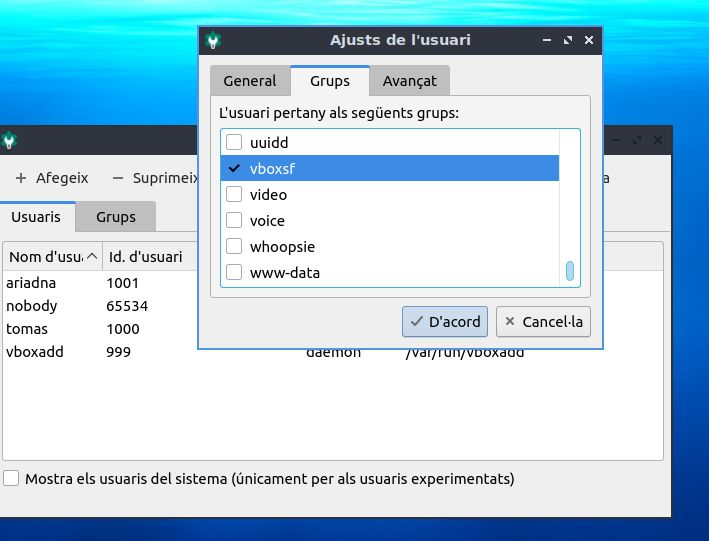
\includegraphics{png/usuarisGUI2.png}
\caption{Figura2:Usuario. Grups}
\end{figure}

\begin{figure}
\centering
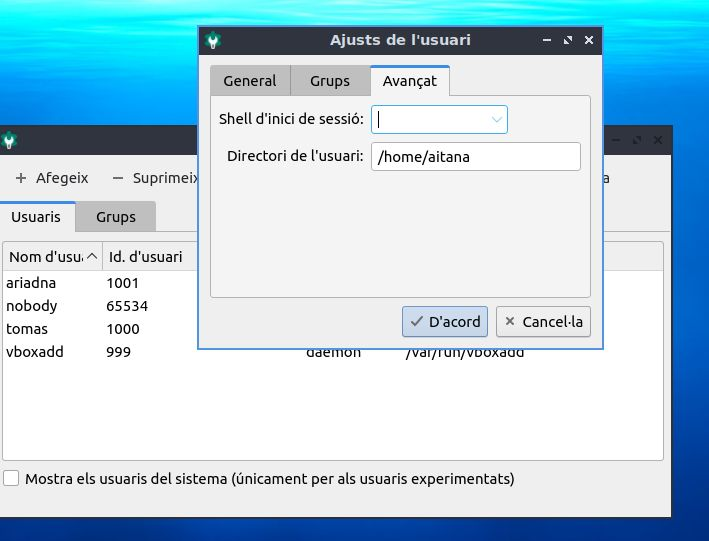
\includegraphics{png/usuarisGUI3.png}
\caption{Figura3:Usuario. Directori de treball i shell}
\end{figure}

\section{4 Gestió des del terminal i fitxers de
configuració}\label{gestiuxf3-des-del-terminal-i-fitxers-de-configuraciuxf3}

Les ordres del terminal tenen avantatges respecte al GUI:

\begin{itemize}
\tightlist
\item
  Molt sovint les opcions gràfiques poden donar problemes.
\item
  Poden automatitzar-se (per exemple, un script que llig un fitxer csv
  on estan els usuaris i els crea tots de colp).
\item
  Podem consultar i modificar (fent còpia de seguretat abans) els
  fitxers de configuració.
\item
  No sempre disposarem de GUI.
\end{itemize}

\subsection{\texorpdfstring{4.1 Alta d'usuari:
\emph{useradd}}{4.1 Alta d'usuari: useradd}}\label{alta-dusuari-useradd}

Creem un usuari ``vicenta'' assignant-li com a grup principal ``tomas''
( paràmetre ``-g'' ).

\begin{itemize}
\tightlist
\item
  -g grup principal
\item
  -G l'afegim a un segon grup
\item
  -s li assignem un shell per defecte
\item
  -c Un descriptor
\item
  -h Directori de treball (home)\ldots{}
\item
  -m \ldots el crea (make) si no existeix
\end{itemize}

La contrassenya s'assigna amb ``passwd''

\begin{Shaded}
\begin{Highlighting}[]
\ExtensionTok{tomas@tomas{-}VirtualBox:\textasciitilde{}$}\NormalTok{ sudo useradd vicenta }\AttributeTok{{-}g}\NormalTok{ grContabilidad }\AttributeTok{{-}m} \AttributeTok{{-}d}\NormalTok{ /home/vta }\AttributeTok{{-}s}\NormalTok{ /bin/bash }\AttributeTok{{-}c} \StringTok{"Vicenta Ferrer"}
\ExtensionTok{tomas@tomas{-}VirtualBox:\textasciitilde{}$}\NormalTok{ sudo useradd vicenta }\AttributeTok{{-}aG}\NormalTok{ grFacturacion}
\ExtensionTok{tomas@tomas{-}VirtualBox:\textasciitilde{}$}\NormalTok{ sudo passwd vicenta}
\ExtensionTok{Nova}\NormalTok{ contrasenya de : }
\ExtensionTok{Torneu}\NormalTok{ a escriure la nova contrasenya de : }
\ExtensionTok{passwd:}\NormalTok{ s}\StringTok{\textquotesingle{}ha actualitzat la contrasenya satisfactòriament}
\StringTok{tomas@tomas{-}VirtualBox:\textasciitilde{}$ }
\end{Highlighting}
\end{Shaded}

Comprovem els grups\ldots{}

\begin{Shaded}
\begin{Highlighting}[]
\ExtensionTok{tomas@tomas{-}VirtualBox:\textasciitilde{}$}\NormalTok{ cat /etc/group}\KeywordTok{|}\FunctionTok{grep}\NormalTok{ Contab}
\ExtensionTok{grContabiliad:x:1002:vicenta}
\ExtensionTok{tomas@tomas{-}VirtualBox:\textasciitilde{}$}\NormalTok{ groups vicenta}
\ExtensionTok{vicenta}\NormalTok{ : grContabilidad grFacturacion}
\end{Highlighting}
\end{Shaded}

\subsection{\texorpdfstring{4.2 Modificació d'usuari:
\emph{usermod}}{4.2 Modificació d'usuari: usermod}}\label{modificaciuxf3-dusuari-usermod}

Com exemple, afegim l'usuari al grup ``rosa''. Compte!, hem d'incloure
els grups secundaris existents si no afegim ``-a''

\begin{Shaded}
\begin{Highlighting}[]
\ExtensionTok{tomas@tomas{-}VirtualBox:\textasciitilde{}$}\NormalTok{ sudo usermod vicenta }\AttributeTok{{-}G}\NormalTok{ rosa,pere}
\end{Highlighting}
\end{Shaded}

Compte! Amb -G hem d'indicar la llista sencera de grups

Observem al fitxer de grups en quants està vicente

\begin{Shaded}
\begin{Highlighting}[]
\ExtensionTok{tomas@tomas{-}VirtualBox:\textasciitilde{}$}\NormalTok{ cat /etc/group}\KeywordTok{|}\FunctionTok{grep}\NormalTok{ vicenta}
\ExtensionTok{grContabilitat:x:1001:vicenta}
\ExtensionTok{grFacturacion:x:1002:vicenta}
\end{Highlighting}
\end{Shaded}

També amb l'ordre \emph{groups}

\begin{Shaded}
\begin{Highlighting}[]
\ExtensionTok{tomas@tomas{-}VirtualBox:\textasciitilde{}$}\NormalTok{ groups vicenta}
\ExtensionTok{vicenta}\NormalTok{ : tomas grContabilidad grFacturacion}
\end{Highlighting}
\end{Shaded}

Amb els paràmetres ``-G'' i ``-aG'' (add)

\begin{Shaded}
\begin{Highlighting}[]
\ExtensionTok{tomas@tomas{-}VirtualBox:\textasciitilde{}$}\NormalTok{ sudo usermod vicenta }\AttributeTok{{-}aG}\NormalTok{ grVendedores}
\end{Highlighting}
\end{Shaded}

\subsection{4.3 PERFIL d'USUARI}\label{perfil-dusuari}

Comprovem que existeix el directori \emph{home} però no conté els
directoris del perfil ``Documents'', ``Baixades''\ldots{} Cal iniciar la
sessió des de l'entorn gràfic.

\begin{Shaded}
\begin{Highlighting}[]
\ExtensionTok{tomas@tomas{-}VirtualBox:\textasciitilde{}$}\NormalTok{ ls /home/vta}
\ExtensionTok{tomas@tomas{-}VirtualBox:\textasciitilde{}$}\NormalTok{ ls /home}
\ExtensionTok{enric}\NormalTok{  pere  rosa  tomas  vta}
\ExtensionTok{tomas@tomas{-}VirtualBox:\textasciitilde{}$} 
\end{Highlighting}
\end{Shaded}

Amb el primer inici de sessió en el PC de l'usuari nou, es crea el
perfil sencer ( carpetes DOcuments, Baixades\ldots)

\begin{quote}
PROPIETARI És molt important que es fixeu en el propietari del
directori, fent \emph{ls -l} o també amb \emph{stat}
\end{quote}

\subsection{\texorpdfstring{4.4 Eliminació:
\emph{userdel}}{4.4 Eliminació: userdel}}\label{eliminaciuxf3-userdel}

Sobre el \emph{userdel} convé conéixer el paràmtre ``-r'' per borrar els
directoris de treball i saber que si el grup principal conté altres
usuaris es manté.

\begin{Shaded}
\begin{Highlighting}[]
\ExtensionTok{tomas@tomas{-}VirtualBox:\textasciitilde{}$}\NormalTok{ sudo userdel }\AttributeTok{{-}r}\NormalTok{ pere}
\ExtensionTok{userdel:}\NormalTok{ no s}\StringTok{\textquotesingle{}eliminarà el grup pere donat que hi ha usuaris assignats.}
\StringTok{userdel: pere no s\textquotesingle{}}\NormalTok{ha trobat la cua de correu }\ErrorTok{(}\ExtensionTok{/var/mail/pere}\KeywordTok{)}
\end{Highlighting}
\end{Shaded}

\subsection{\texorpdfstring{4.5 Alta de grups:
\emph{groupadd}}{4.5 Alta de grups: groupadd}}\label{alta-de-grups-groupadd}

Ja hem vist com assignar usuaris a grups amb ``usermod'' veiem ara
ordres de grups.

\begin{Shaded}
\begin{Highlighting}[]
\ExtensionTok{tomas@tomas{-}VirtualBox:\textasciitilde{}$}\NormalTok{ sudo groupadd gr1}
\ExtensionTok{[sudo]}\NormalTok{ contrasenya per a tomas: }
\ExtensionTok{tomas@tomas{-}VirtualBox:\textasciitilde{}$}\NormalTok{ sudo groupadd }\AttributeTok{{-}r}\NormalTok{ gr2}
\end{Highlighting}
\end{Shaded}

\subsection{\texorpdfstring{4.6 Eliminació de grups:
\emph{groupdel}}{4.6 Eliminació de grups: groupdel}}\label{eliminaciuxf3-de-grups-groupdel}

\begin{Shaded}
\begin{Highlighting}[]
\ExtensionTok{tomas@tomas{-}VirtualBox:\textasciitilde{}$}\NormalTok{ sudo useradd  }\AttributeTok{{-}g}\NormalTok{ gr1 joana}
\ExtensionTok{tomas@tomas{-}VirtualBox:\textasciitilde{}$}\NormalTok{ sudo groupdel gr1}
\ExtensionTok{groupdel:}\NormalTok{ no es pot eliminar el grup primari de l}\StringTok{\textquotesingle{}usuari «joana»}
\end{Highlighting}
\end{Shaded}

\subsection{4.7 Administració dels
grups}\label{administraciuxf3-dels-grups}

Afegir un usuari a un grup. Veiem les dos alternatives:

\begin{itemize}
\item
  amb el gpasswd -a
\item
  amb el usermod -a -G
\end{itemize}

Per a eliminar un usuari del grup. Veiem les dos alternatives:

\begin{itemize}
\item
  amb el gpasswd -d
\item
  amb el usermod -G ( indicant els grups excepte el que volem llevar )
\end{itemize}

(l'opció -G té el perill d'oblidar-nos-en d'algun grup!)

Al següent exemple afegim enric a gr2, l'eliminem i el tornem a afegir.

\begin{Shaded}
\begin{Highlighting}[]
\ExtensionTok{tomas@tomas{-}VirtualBox:\textasciitilde{}$}\NormalTok{ sudo gpasswd }\AttributeTok{{-}a}\NormalTok{ enric gr2}
\ExtensionTok{S}\StringTok{\textquotesingle{}està afegint l\textquotesingle{}}\ExtensionTok{usuari}\NormalTok{ enric al grup gr2}
\ExtensionTok{tomas@tomas{-}VirtualBox:\textasciitilde{}$}\NormalTok{ sudo gpasswd }\AttributeTok{{-}d}\NormalTok{ enric gr2}
\ExtensionTok{S}\StringTok{\textquotesingle{}està eliminant l\textquotesingle{}}\ExtensionTok{usuari}\NormalTok{ enric del grup gr2}
\ExtensionTok{tomas@tomas{-}VirtualBox:\textasciitilde{}$}\NormalTok{ sudo usermod enric }\AttributeTok{{-}a} \AttributeTok{{-}G}\NormalTok{ gr2}
\end{Highlighting}
\end{Shaded}

\emph{(NO solen usar-se contrassenyes de grup. No estudiar)} Afegir i
eliminar contrasenya al grup

\begin{Shaded}
\begin{Highlighting}[]
\FunctionTok{sudo}\NormalTok{ gpasswd gr1}
\end{Highlighting}
\end{Shaded}

\begin{Shaded}
\begin{Highlighting}[]
\FunctionTok{sudo}\NormalTok{ gpasswd }\AttributeTok{{-}r}\NormalTok{ gr1}
\end{Highlighting}
\end{Shaded}

El fitxer de contrassenyes encriptades de grup\ldots{}

\begin{Shaded}
\begin{Highlighting}[]
\NormalTok{sudo cat/etc/gshadow}
\NormalTok{...}
\NormalTok{...}
\NormalTok{gr1:::}
\NormalTok{gr2:!::enric}
\end{Highlighting}
\end{Shaded}

\section{5 Resum: Fitxers de configuració dels comptes
locals.}\label{resum-fitxers-de-configuraciuxf3-dels-comptes-locals.}

En el present curs (SOM) ens centrarem en els dos primers.

\begin{longtable}[]{@{}
  >{\raggedright\arraybackslash}p{(\columnwidth - 4\tabcolsep) * \real{0.1549}}
  >{\raggedright\arraybackslash}p{(\columnwidth - 4\tabcolsep) * \real{0.4859}}
  >{\raggedright\arraybackslash}p{(\columnwidth - 4\tabcolsep) * \real{0.3592}}@{}}
\toprule\noalign{}
\begin{minipage}[b]{\linewidth}\raggedright
\textbf{Fitxer}
\end{minipage} & \begin{minipage}[b]{\linewidth}\raggedright
\textbf{Funció}
\end{minipage} & \begin{minipage}[b]{\linewidth}\raggedright
\textbf{Exemple de Contingut}
\end{minipage} \\
\midrule\noalign{}
\endhead
\bottomrule\noalign{}
\endlastfoot
\textbf{/etc/passwd} & Informació bàsica dels usuaris (UID, directori
inicial, shell). & \texttt{user:x:1001:1001:/home/user:/bin/bash} \\
\textbf{/etc/group} & Informació dels grups (GID, membres). &
\texttt{group:x:1001:user1,user2} \\
\textbf{/etc/shadow} & Contrasenyes encriptades i configuració de
caducitat. & \texttt{user:\$6\$...:19000:0:99999:7:::} \\
\textbf{/etc/gshadow} & Configuració avançada de grups (inclou
contrasenyes de grup). & \texttt{group:!:1001:user1,user2} \\
\textbf{/etc/login.defs} & Paràmetres globals per usuaris (expiració de
contrasenyes, UID/GID). & \texttt{PASS\_MAX\_DAYS\ 90} \\
\textbf{/etc/default/useradd} & Configuració predeterminada per nous
usuaris. & \texttt{SHELL=/bin/bash} \\
\textbf{/etc/skel/} & Plantilla per als nous usuaris (fitxers inicials).
& \texttt{.bashrc}, \texttt{.profile} \\
\textbf{/etc/security/limits.conf} & Límits de recursos per als usuaris.
& \texttt{user\ hard\ nofile\ 1024} \\
\textbf{/etc/security/pwquality.conf} & Complexitat de la contrassenya
& \\
\textbf{/etc/pam.d/common-password} & Fitxer associat a la configuració
de contrassenyes & \\
\end{longtable}

\section{6 Els UID i GID}\label{els-uid-i-gid}

En sistemes Ubuntu, els \textbf{UID} (User ID) i \textbf{GID} (Group ID)
es divideixen en intervals segons els tipus de comptes.

\begin{longtable}[]{@{}
  >{\raggedright\arraybackslash}p{(\columnwidth - 4\tabcolsep) * \real{0.2093}}
  >{\raggedright\arraybackslash}p{(\columnwidth - 4\tabcolsep) * \real{0.1783}}
  >{\raggedright\arraybackslash}p{(\columnwidth - 4\tabcolsep) * \real{0.6124}}@{}}
\toprule\noalign{}
\begin{minipage}[b]{\linewidth}\raggedright
\textbf{Tipus de Compte}
\end{minipage} & \begin{minipage}[b]{\linewidth}\raggedright
\textbf{Interval UID/GID}
\end{minipage} & \begin{minipage}[b]{\linewidth}\raggedright
\textbf{Descripció}
\end{minipage} \\
\midrule\noalign{}
\endhead
\bottomrule\noalign{}
\endlastfoot
\textbf{Usuaris del sistema} & 0--999 & Comptes reservats per al sistema
i serveis. Inclou l'usuari \texttt{root} (UID 0). \\
\textbf{Usuaris normals} & 1000--59999 & Comptes creats per usuaris
humans (per defecte, comença a 1000). \\
\textbf{UID dinàmics} & 60000--65533 & Reservat per a comptes temporals
o dinàmics (normalment creats per processos). \\
\end{longtable}

Podríem modificar-los manualment amb nano \emph{/etc/login.defs}, sempre
fent una còpia prèvia!

\end{document}
